\documentclass[conference]{IEEEtran}
\usepackage{amsmath,amssymb,amsthm}
\usepackage{graphicx}
\usepackage{booktabs}
\usepackage{cite}
\usepackage[hidelinks]{hyperref}
\graphicspath{{figures/}}
\pdfminorversion=4

\newtheorem{proposition}{Proposition}
\newcommand{\bv}[1]{\mathbf{#1}}
\newcommand{\Jm}{\boldsymbol{\mathcal{J}}}

\begin{document}

\title{Flatness-Based and Passivity-Based Control with Adaptive RBF Neural Compensation of a 2~MW Direct-Drive PMSG Wind Energy Conversion System}

\author{
\IEEEauthorblockN{Said Regani}
\IEEEauthorblockA{\textit{L2EI Laboratory}\\
\textit{Jijel University}\\
BP 98 Ouled Aissa, Jijel 18000, Algeria}
\and
\IEEEauthorblockN{Manal Messadi}
\IEEEauthorblockA{\textit{L2EI Laboratory}\\
\textit{Jijel University}\\
BP 98 Ouled Aissa, Jijel 18000, Algeria}
\and
\IEEEauthorblockN{Kemih Karim}
\IEEEauthorblockA{\textit{L2EI Laboratory}\\
\textit{Jijel University}\\
BP 98 Ouled Aissa, Jijel 18000, Algeria}
}

\maketitle

\begin{abstract}
This paper presents the modeling and control of a 2~MW direct-drive wind energy conversion system
based on a permanent magnet synchronous generator (PMSG) connected to the grid through a back-to-back
converter and an $L$ filter. The generator is modeled in the receptor convention, and the signs of the
complete model are verified by an exact power balance. The rotor speed and the energy stored in the DC
link and in the filter are used as flat outputs of the two outer loops, and the currents of both
converters are controlled by passivity-based control (PBC). A radial basis function (RBF) neural
network, adapted online by a Lyapunov law with $\sigma$-modification, compensates the uncertainty of
the aerodynamic-torque model and of the generator parameters. Simulations with step and turbulent wind,
parameter mismatch and a 50\,\% grid voltage dip show that all the controlled variables track their
references, that the DC-link voltage remains within 1.7~V of 1200~V outside the dip, and that the
neural compensation reduces the integral absolute speed error by 27 to 49\,\%.
\end{abstract}

\begin{IEEEkeywords}
PMSG, wind energy conversion, flatness, passivity-based control, RBF neural network, back-to-back converter.
\end{IEEEkeywords}

\section{Introduction}
Wind energy is one of the main sources in the transition towards low-carbon electricity
generation~\cite{iea2024,gwec2024}. Direct-drive PMSG turbines remove the gearbox, which reduces
maintenance and losses, and their full-scale back-to-back converter decouples the generator from the
grid~\cite{polinder2013,wu2011}. The machine-side converter (MSC) controls the generator torque to track
the maximum power point, and the grid-side converter (GSC) regulates the DC-link voltage and injects the
power into the grid.

These tasks are usually performed by cascaded PI loops in rotating frames~\cite{chinchilla2006,yazdani2010}.
Differential flatness~\cite{fliess1995} computes the control directly from the desired trajectory of a
flat output and has been applied to the PMSG wind turbine and its DC link~\cite{aimene2022}; with the
stored energy as flat output, the DC-link dynamics become a linear power balance~\cite{thounthong2010}.
Passivity-based control~\cite{ortega1998} shapes the energy of the closed loop and keeps the workless
coupling terms of electrical machines. Both methods use a model; their weak point is the aerodynamic
torque, which is not measured, and the parameter uncertainty, which neural networks can learn
online~\cite{lewis1999}.

This paper presents:
\begin{itemize}
\item a complete model of a 2~MW direct-drive PMSG wind energy conversion system in the receptor
convention, with an exact power balance that verifies its signs;
\item flat outer loops for the rotor speed and the DC-link energy, and PBC current loops for both
converters;
\item an RBF network that compensates the aerodynamic-torque and parameter uncertainty in the flat speed
law, with a Lyapunov stability proof;
\item simulation results without and with the neural compensation under step and turbulent wind,
parameter mismatch and a grid voltage dip.
\end{itemize}

\section{System Modeling}
The studied system is shown in Fig.~\ref{fig:system}. The turbine drives the PMSG directly; the MSC
rectifies the generator voltages, the DC link decouples the two converters, and the GSC injects the
power into the 690~V, 50~Hz grid through an $L$ filter.

\begin{figure}[t]
\centering
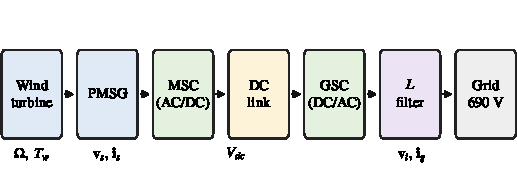
\includegraphics[width=\columnwidth]{system.pdf}
\caption{Direct-drive PMSG wind energy conversion system with a back-to-back converter.}
\label{fig:system}
\end{figure}

\subsection{Wind Speed}
Two wind profiles are used. The step profile (9~m/s, 11~m/s at 10~s and 8~m/s at 25~s), similar to
the one of~\cite{aimene2022}, assesses the transient response. The turbulent profile is
\begin{equation}
v(t) = V_m + \textstyle\sum_{k=1}^{3} A_k\sin(2\pi f_k t) + v_t(t)
\label{eq:wind}
\end{equation}
with $V_m=8.5$~m/s, $A=[1.5,\,0.2,\,0.3]$~m/s and $f=[0.03,\,0.16,\,0.17]$~Hz~\cite{regani2026}; the
turbulence $v_t$ is a first-order coloured noise with a standard deviation of 0.5~m/s and a correlation
time of 1.5~s. Over 40~s, the wind remains between 6.0 and 10.9~m/s, below the rated wind speed, so the
pitch angle is zero. The controller uses the anemometer measurement $v_m$, modeled by a first-order lag
of 1~s.

\subsection{Wind Turbine}
The power captured by the rotor and the tip-speed ratio are~\cite{heier2014,aimene2022}
\begin{equation}
P_w = \tfrac{1}{2}\rho\pi R^2 C_p(\lambda,\beta)\,v^3,\qquad \lambda=\frac{\Omega R}{v}
\label{eq:pw}
\end{equation}
where $\rho$ is the air density, $R$ the rotor radius, $\Omega$ the rotor speed and $\beta$ the pitch
angle. The power coefficient is
\begin{equation}
C_p = 0.5176\Bigl(\frac{116}{\lambda_i}-0.4\beta-5\Bigr)e^{-21/\lambda_i}+0.0068\lambda,
\label{eq:cp}
\end{equation}
with $1/\lambda_i=1/(\lambda+0.08\beta)-0.035/(\beta^3+1)$. For $\beta=0$, $C_{p,\max}=0.48$ at
$\lambda_{opt}=8.1$ (Fig.~\ref{fig:turbine}). The aerodynamic torque is $T_w=P_w/\Omega$. For
$P_n=2$~MW and $R=40$~m, close to the 2~MW turbine of~\cite{rolan2009}, the rated wind speed given by
$P_n=\frac12\rho\pi R^2C_{p,\max}v_n^3$ is $v_n=11.0$~m/s, the rated speed is
$\Omega_n=\lambda_{opt}v_n/R=2.23$~rad/s and the rated torque is $T_n=P_n/\Omega_n=0.897$~MN$\cdot$m.

\begin{figure}[t]
\centering
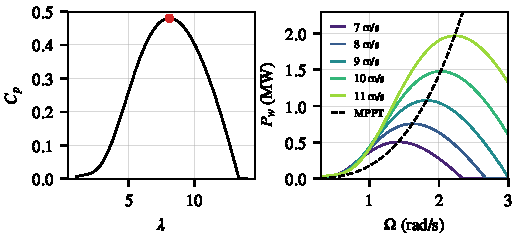
\includegraphics[width=\columnwidth]{turbine.pdf}
\caption{Power coefficient for $\beta=0$ (left) and captured power versus rotor speed with the maximum
power curve (right).}
\label{fig:turbine}
\end{figure}

\subsection{Shaft}
The direct-drive shaft is described by the one-mass model
\begin{equation}
J\frac{d\Omega}{dt} = T_w + T_e - B\Omega
\label{eq:shaft}
\end{equation}
where $J$ is the total inertia, $B$ the friction coefficient and $T_e$ the electromagnetic torque in the
receptor convention ($T_e<0$ in generating mode).

\subsection{PMSG}
In the rotor $dq$ frame (amplitude-invariant transformation, $d$ axis on the magnet flux), with the
receptor convention and $L_d=L_q=L_s$~\cite{aimene2022},
\begin{align}
v_{sd} &= R_s i_{sd} + L_s\frac{di_{sd}}{dt} - \omega_e L_s i_{sq}\label{eq:vsd}\\
v_{sq} &= R_s i_{sq} + L_s\frac{di_{sq}}{dt} + \omega_e L_s i_{sd} + \omega_e\psi_f\label{eq:vsq}\\
T_e &= \tfrac32 p\,\psi_f\, i_{sq}\label{eq:te}
\end{align}
where $\omega_e=p\Omega$, $p$ is the number of pole pairs and $\psi_f$ the magnet flux. With
$\bv{i}_s=[i_{sd}\;i_{sq}]^T$, $\bv{v}_s=[v_{sd}\;v_{sq}]^T$, $\bv{e}_q=[0\;1]^T$ and the skew-symmetric
matrix $\Jm=\bigl[\begin{smallmatrix}0&1\\-1&0\end{smallmatrix}\bigr]$,
\begin{equation}
L_s\dot{\bv{i}}_s = \bv{v}_s - R_s\bv{i}_s + \omega_eL_s\Jm\bv{i}_s - \omega_e\psi_f\bv{e}_q .
\label{eq:pmsg}
\end{equation}
The generator data are those of the non-salient 2~MW PMSG of~\cite{hasan2021} (Table~\ref{tab:param}):
at $\Omega_n$, the back-EMF $p\Omega_n\psi_f=532$~V is close to the peak phase voltage of the grid
(563~V).

\subsection{Back-to-Back Converter and DC Link}
The two-level converters are represented by their average model, with voltage vectors limited to
$V_{dc}/\sqrt3$. The DC link receives the power of the MSC and supplies the GSC~\cite{aimene2022}:
\begin{equation}
CV_{dc}\frac{dV_{dc}}{dt} = P_{dc} - P_i,\quad P_{dc}=-\tfrac32\bv{v}_s^T\bv{i}_s,\quad
P_i=\tfrac32\bv{v}_i^T\bv{i}_g .
\label{eq:dc}
\end{equation}

\subsection{$L$ Filter and Grid}
In the grid-voltage-oriented frame ($v_{gq}=0$, ideal PLL), with the current counted towards the
grid~\cite{aimene2022},
\begin{equation}
L_f\dot{\bv{i}}_g = \bv{v}_i - R_f\bv{i}_g + \omega_gL_f\Jm\bv{i}_g - \bv{v}_g ,
\label{eq:filter}
\end{equation}
and the grid powers are $P_g=\frac32v_{gd}i_{gd}$ and $Q_g=-\frac32v_{gd}i_{gq}$.

\subsection{Power Balance}
With $E=\frac12J\Omega^2+\frac34L_s\|\bv{i}_s\|^2+\frac12CV_{dc}^2+\frac34L_f\|\bv{i}_g\|^2$, and since
$\bv{x}^T\Jm\bv{x}=0$ and $T_e\Omega=\frac32\omega_e\psi_fi_{sq}$, the model gives, for any state and
converter voltages,
\begin{equation}
\dot E = P_w - B\Omega^2 - \tfrac32R_s\|\bv{i}_s\|^2 - \tfrac32R_f\|\bv{i}_g\|^2 - P_g ,
\label{eq:balance}
\end{equation}
which verifies the sign of every term; its numerical residual is below $10^{-15}P_n$.

\begin{table}[t]
\caption{Parameters of the Studied System}
\label{tab:param}
\centering
\footnotesize
\setlength{\tabcolsep}{3pt}
\begin{tabular}{llll}
\toprule
Parameter & Symbol & Value & Source\\
\midrule
Rated power & $P_n$ & 2 MW & \cite{hasan2021}\\
Rotor radius & $R$ & 40 m & \cite{rolan2009}\\
Air density & $\rho$ & 1.225 kg/m$^3$ & \cite{aimene2022}\\
Rated wind / rotor speed & $v_n$, $\Omega_n$ & 11.0 m/s, 2.23 rad/s & (\ref{eq:pw})\\
Total inertia & $J$ & $2.8\times10^6$ kg$\cdot$m$^2$ & assumed\\
Friction coefficient & $B$ & $10^3$ N$\cdot$m$\cdot$s & assumed\\
Pole pairs & $p$ & 26 & \cite{hasan2021}\\
Stator resistance & $R_s$ & 0.78 m$\Omega$ & \cite{hasan2021}\\
Stator inductance & $L_s$ & 1.57 mH & \cite{hasan2021}\\
Magnet flux & $\psi_f$ & 9.18 Wb & \cite{hasan2021}\\
DC link & $C$, $V_{dc}^*$ & 20 mF, 1200 V & \cite{hasan2021}\\
Filter & $L_f$, $R_f$ & 0.15 mH, 2 m$\Omega$ & \cite{hasan2021}, assumed\\
Grid & & 690 V, 50 Hz & \cite{hasan2021}\\
Switching frequency & $f_{sw}$ & 2160 Hz & \cite{hasan2021}\\
\bottomrule
\end{tabular}
\end{table}

\section{Control}
The control structure is shown in Fig.~\ref{fig:structure}. All errors are defined as measured minus
reference values. The controller is sampled at $T_s=1/(2f_{sw})=231.5~\mu$s, and the converter voltages
are applied one sample after their computation.

\begin{figure}[t]
\centering
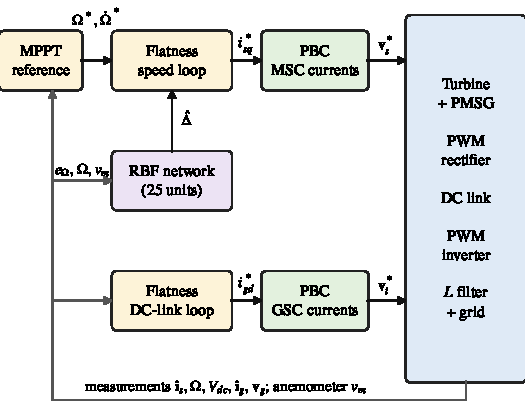
\includegraphics[width=0.92\columnwidth]{structure.pdf}
\caption{Control structure: flat outer loops, PBC current loops and RBF compensation.}
\label{fig:structure}
\end{figure}

\subsection{MPPT Reference}
The optimal speed $\Omega_{opt}=\lambda_{opt}v_m/R$, limited to $[0.5\Omega_n,\Omega_n]$, is filtered by
$\ddot\Omega^*=\omega_r^2(\Omega_{opt}-\Omega^*)-2\omega_r\dot\Omega^*$ ($\omega_r=1$~rad/s), which
gives a smooth reference $\Omega^*$ and its derivative.

\subsection{Flatness-Based Speed Loop}
From (\ref{eq:shaft}), $T_e=J\dot\Omega+B\Omega-T_w$: $\Omega$ is a flat output of the shaft with input
$T_e$, i.e., $i_{sq}$~\cite{fliess1995,aimene2022}. Imposing $\dot\Omega=\nu_1$ with
$\nu_1=\dot\Omega^*-k_{11}e_\Omega-k_{12}\!\int\!e_\Omega dt$, $e_\Omega=\Omega-\Omega^*$, gives
\begin{equation}
T_e^* = J\nu_1 + B\Omega - \hat T_w - \hat\Delta,\qquad i_{sq}^*=\frac{T_e^*}{\frac32p\psi_f},\quad i_{sd}^*=0
\label{eq:flat1}
\end{equation}
where $\hat T_w$ is computed from (\ref{eq:pw})--(\ref{eq:cp}) with $v_m$, and $\hat\Delta$ is the neural
compensation ($\hat\Delta=0$ without the network). $T_e^*$ is limited to $[-1.2T_n,0]$, with the
integration frozen at the limit. With $i_{sq}=i_{sq}^*$ and $\Delta=T_w-\hat T_w$,
\begin{equation}
J\bigl(\dot e_\Omega + k_{11}e_\Omega + k_{12}\!\textstyle\int\! e_\Omega dt\bigr) = \Delta-\hat\Delta .
\label{eq:errw}
\end{equation}

\subsection{Flatness-Based DC-Link Loop}
The flat output is the energy of the DC link and of the filter,
$y_2=\frac12CV_{dc}^2+\frac34L_f\|\bv{i}_g\|^2$. From (\ref{eq:dc})--(\ref{eq:filter}),
\begin{equation}
\dot y_2 = P_{dc} - P_g - \tfrac32R_f\|\bv{i}_g\|^2 ,
\label{eq:y2}
\end{equation}
which is linear in the grid power~\cite{thounthong2010}. Imposing $\dot y_2=-k_{21}e_y-k_{22}\int e_y\,dt$,
with $e_y=y_2-y_2^*$ and $y_2^*=\frac12CV_{dc}^{*2}+\frac34L_f\|\bv{i}_g^*\|^2$, gives
\begin{equation}
P_g^* = P_{dc} - \tfrac32R_f\|\bv{i}_g\|^2 + k_{21}e_y + k_{22}\!\int\! e_y dt,\quad
i_{gd}^*=\frac{2P_g^*}{3v_{gd}}
\label{eq:flat2}
\end{equation}
and $i_{gq}^*=0$ (unity power factor). $P_{dc}$ is computed from the applied MSC voltages and the measured
currents, so the generator power is passed to the grid before it changes $V_{dc}$.

\subsection{Passivity-Based Current Loops}
With $\bv{e}_s=\bv{i}_s-\bv{i}_s^*$ and $\dot{\bv{z}}_s=\bv{e}_s$, the MSC voltage reference is
\begin{equation}
\bv{v}_s^* = L_s\dot{\bv{i}}_s^* + R_s\bv{i}_s^* - \omega_eL_s\Jm\bv{i}_s^* + \omega_e\psi_f\bv{e}_q
- R_a\bv{e}_s - K_i\bv{z}_s
\label{eq:pbc1}
\end{equation}
and, with $\bv{e}_g=\bv{i}_g-\bv{i}_g^*$ and $\dot{\bv{z}}_g=\bv{e}_g$, the GSC voltage reference is
\begin{equation}
\bv{v}_i^* = L_f\dot{\bv{i}}_g^* + R_f\bv{i}_g^* - \omega_gL_f\Jm\bv{i}_g^* + \bv{v}_g
- R_b\bv{e}_g - K_{ig}\bv{z}_g .
\label{eq:pbc2}
\end{equation}
The reference derivatives are obtained by first-order filters (2~ms), and the integrals are frozen when
the voltage reaches $V_{dc}/\sqrt3$.

\begin{proposition}
With (\ref{eq:pbc1}) applied to (\ref{eq:pmsg}) and $R_a,K_i>0$, the storage function
$H=\frac12L_s\|\bv{e}_s\|^2+\frac12K_i\|\bv{z}_s\|^2$ satisfies $\dot H=-(R_s+R_a)\|\bv{e}_s\|^2$ and
$\bv{e}_s\to0$. The same holds for (\ref{eq:pbc2}) applied to (\ref{eq:filter}).
\end{proposition}
\begin{proof}
Subtracting $L_s\dot{\bv{i}}_s^*$ from (\ref{eq:pmsg}) and inserting (\ref{eq:pbc1}) gives
$L_s\dot{\bv{e}}_s=-(R_s+R_a)\bv{e}_s+\omega_eL_s\Jm\bv{e}_s-K_i\bv{z}_s$. Hence
$\dot H=\bv{e}_s^TL_s\dot{\bv{e}}_s+K_i\bv{z}_s^T\bv{e}_s=-(R_s+R_a)\|\bv{e}_s\|^2$, since
$\bv{e}_s^T\Jm\bv{e}_s=0$. $H$ is bounded and $\dot H$ is uniformly continuous, so Barbalat's
lemma~\cite{khalil2002} gives $\bv{e}_s\to0$.
\end{proof}

\subsection{Adaptive RBF Compensation}
The uncertainty $\Delta=T_w-\hat T_w$, due to the $C_p$ model, the anemometer and the generator
parameters, is approximated on the operating region by $\Delta=\bv{W}^{*T}\boldsymbol\phi(\bv{z})+\varepsilon$,
$|\varepsilon|\le\bar\varepsilon$, with $\bv{z}=[\Omega/\Omega_n,\;v_m/v_n]^T$ and 25 Gaussian functions
$\phi_j=\exp(-\|\bv{z}-\bv{c}_j\|^2/(2b^2))$ centred on a $5\times5$ grid of $[0.5,1.1]^2$, $b=0.15$.
The compensation $\hat\Delta=\hat{\bv{W}}^T\boldsymbol\phi$ replaces the integral of the speed loop
($k_{12}=0$ when the network is used) and is adapted by
\begin{equation}
\dot{\hat{\bv{W}}} = \Gamma\bigl(\boldsymbol\phi\,e_\Omega - \sigma\hat{\bv{W}}\bigr),
\label{eq:law}
\end{equation}
frozen when $T_e^*$ saturates, with $\hat{\bv{W}}(0)=0$.

\begin{proposition}
Consider (\ref{eq:errw}) with $k_{12}=0$ and the law (\ref{eq:law}) with $\Gamma,\sigma>0$, exact $J$
and $B$, and no saturation. Then $e_\Omega$ and $\tilde{\bv{W}}=\bv{W}^*-\hat{\bv{W}}$ are uniformly
ultimately bounded.
\end{proposition}
\begin{proof}
With $V=\frac12Je_\Omega^2+\frac{1}{2\Gamma}\|\tilde{\bv{W}}\|^2$ and (\ref{eq:errw}),
$\dot V=-Jk_{11}e_\Omega^2+e_\Omega(\tilde{\bv{W}}^T\boldsymbol\phi+\varepsilon)
-\frac1\Gamma\tilde{\bv{W}}^T\dot{\hat{\bv{W}}}=-Jk_{11}e_\Omega^2+e_\Omega\varepsilon
+\sigma\tilde{\bv{W}}^T\hat{\bv{W}}$. Using
$\tilde{\bv{W}}^T\hat{\bv{W}}\le\frac12\|\bv{W}^*\|^2-\frac12\|\tilde{\bv{W}}\|^2$ and
$e_\Omega\varepsilon\le\frac{Jk_{11}}{2}e_\Omega^2+\frac{\bar\varepsilon^2}{2Jk_{11}}$ gives
$\dot V\le-\frac{Jk_{11}}{2}e_\Omega^2-\frac\sigma2\|\tilde{\bv{W}}\|^2
+\frac{\bar\varepsilon^2}{2Jk_{11}}+\frac\sigma2\|\bv{W}^*\|^2$, which is negative outside a compact set.
\end{proof}

\begin{table}[t]
\caption{Controller Parameters}
\label{tab:ctrl}
\centering
\footnotesize
\begin{tabular}{ll}
\toprule
Loop & Parameters\\
\midrule
Speed (flat) & $\omega_\Omega=2$ rad/s ($k_{11}=4$, $k_{12}=4$), $\omega_r=1$ rad/s\\
DC link (flat) & $\omega_v=60$ rad/s ($k_{21}=120$, $k_{22}=3600$)\\
PBC MSC & $\omega_i=500$ rad/s: $R_a=1.57~\Omega$, $K_i=393~\Omega$/s\\
PBC GSC & $\omega_i=500$ rad/s: $R_b=0.148~\Omega$, $K_{ig}=37.5~\Omega$/s\\
RBF network & 25 units, $b=0.15$, $\Gamma=10^7$, $\sigma=0.02$ s$^{-1}$\\
\bottomrule
\end{tabular}
\end{table}

The gains place double closed-loop poles: $k_{11}=2\omega_\Omega$, $k_{12}=\omega_\Omega^2$,
$k_{21}=2\omega_v$, $k_{22}=\omega_v^2$, $R_s+R_a=2\omega_iL_s$, $K_i=\omega_i^2L_s$,
$R_f+R_b=2\omega_iL_f$, $K_{ig}=\omega_i^2L_f$ (Table~\ref{tab:ctrl}).

\section{Simulation Results}
\subsection{Setup}
The model is integrated with a fourth-order Runge--Kutta scheme at the step $T_s$ over 40~s, starting
from the MPPT equilibrium. Three cases are considered: (i) step wind with nominal parameters;
(ii) turbulent wind with nominal parameters; (iii) robustness: turbulent wind, true plant with
$C_p\times1.1$, $J\times1.2$, $R_s\times1.5$, $L_s\times1.2$, $\psi_f\times0.95$, $R_f\times1.5$,
$L_f\times1.25$, and a 50\,\% grid voltage dip between 25 and 25.15~s. The proposed control is
evaluated without the network ($\hat\Delta=0$, integral action in the speed loop) and with the network.

\begin{figure*}[t]
\centering
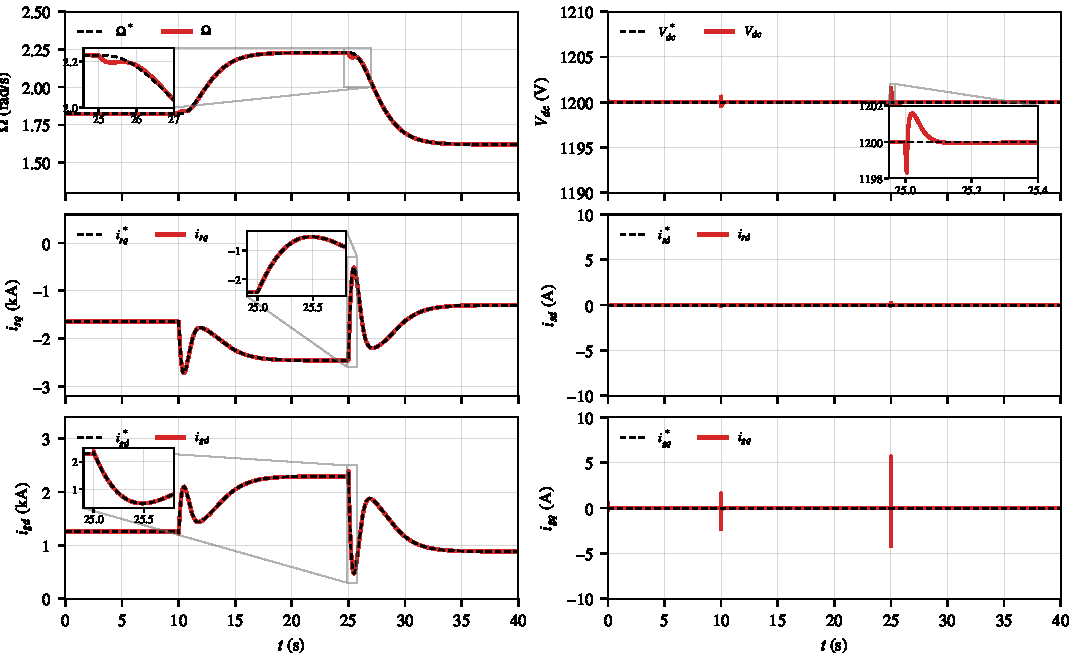
\includegraphics[width=\textwidth]{tracking_step.pdf}
\caption{Step wind, control with the RBF network: references (dashed) and measured values (solid) of the
rotor speed, DC-link voltage and stator and grid currents, with zooms on the step at 25~s.}
\label{fig:track}
\end{figure*}

\subsection{Step Wind}
Fig.~\ref{fig:track} shows that all the controlled variables follow their references. The rotor speed
follows the MPPT reference from 1.82 to 2.23 and 1.62~rad/s; $i_{sq}$ and $i_{gd}$ follow their
references during the transients, $i_{sd}$ and $i_{gq}$ remain at zero, and $V_{dc}$ stays within
1.7~V of 1200~V, since the generator power is passed to the grid through $P_{dc}$ in (\ref{eq:flat2}).

\subsection{Turbulent Wind and Robustness}
Fig.~\ref{fig:mppt} shows the robustness case. The rotor speed follows its reference, and $C_p$ stays
close to its maximum, except during the fast wind decrease around 22~s, where the inertia prevents the
rotor from slowing down quickly. The MPPT efficiency, i.e., the ratio between the captured energy and
the maximum available energy, is 97.7\,\%.

\begin{figure}[t]
\centering
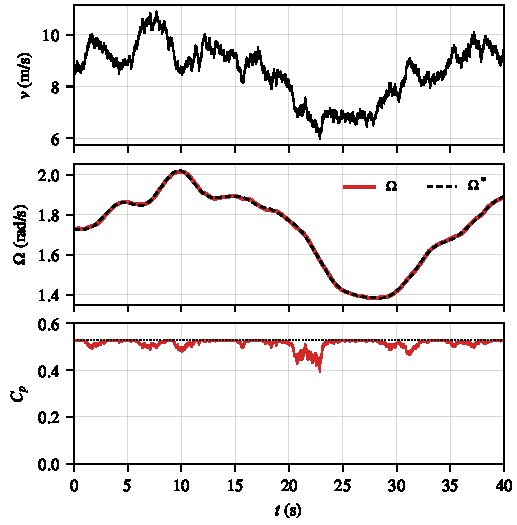
\includegraphics[width=\columnwidth]{mppt.pdf}
\caption{Robustness case with the RBF network: wind speed, rotor speed and reference, and power
coefficient (dotted: $C_{p,\max}$ of the true turbine).}
\label{fig:mppt}
\end{figure}

\subsection{Effect of the Neural Compensation}
Table~\ref{tab:res} and Fig.~\ref{fig:ann} compare the control without and with the network. The network
reduces the IAE of the speed by 49\,\% for the step wind, 27\,\% for the turbulent wind and 29\,\% in the
robustness case: after each wind step, the speed error vanishes in 2 to 3~s instead of 5 to 7~s. The
network estimate follows the actual uncertainty, about 82~kN$\cdot$m on average in the robustness case
(Fig.~\ref{fig:grid}). The current errors and the DC-link deviation are practically unchanged, and the
captured energy is the same; the price is a slightly more active torque (11--14\,\% larger standard
deviation of its rate).

\begin{figure}[t]
\centering
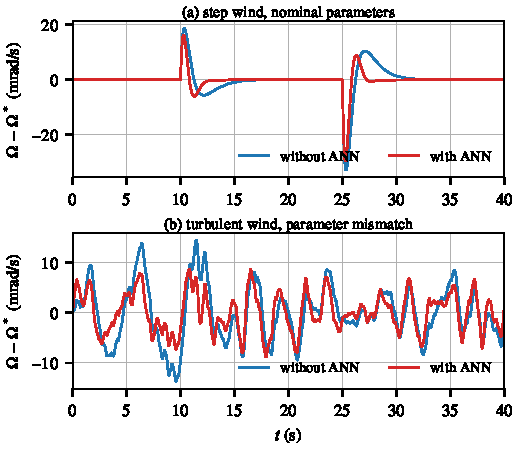
\includegraphics[width=\columnwidth]{ann_effect.pdf}
\caption{Speed tracking error without and with the RBF network: (a) step wind; (b) robustness case.}
\label{fig:ann}
\end{figure}

\begin{table}[t]
\caption{Results Without and With the RBF Network (40 s, from $t=1$ s)}
\label{tab:res}
\centering
\footnotesize
\setlength{\tabcolsep}{2.5pt}
\begin{tabular}{lcccccc}
\toprule
 & \multicolumn{2}{c}{Step} & \multicolumn{2}{c}{Turbulent} & \multicolumn{2}{c}{Robustness}\\
Metric & w/o & with & w/o & with & w/o & with\\
\midrule
IAE of $\Omega$ (rad) & 0.074 & \textbf{0.037} & 0.144 & \textbf{0.105} & 0.177 & \textbf{0.126}\\
RMS $e_{isq}$ (A) & 0.037 & 0.036 & 0.043 & 0.041 & 0.047 & 0.044\\
Max $|V_{dc}-V_{dc}^*|$ (V)$^{a}$ & 1.70 & 1.67 & 0.16 & 0.16 & 0.24 & 0.25\\
Energy (kWh) & 13.86 & 13.86 & 10.05 & 10.04 & 10.98 & 10.97\\
MPPT efficiency (\%) & 98.0 & 98.0 & 97.7 & 97.7 & 97.7 & 97.7\\
Torque rate std (MN$\cdot$m/s) & 0.218 & 0.247 & 0.187 & 0.207 & 0.187 & 0.212\\
\bottomrule
\multicolumn{7}{l}{$^{a}$ outside the grid voltage dip.}
\end{tabular}
\end{table}

\subsection{Grid Voltage Dip}
During the 50\,\% dip (Fig.~\ref{fig:grid}), the grid current doubles to keep the injected power, and
the DC-link voltage deviates by 14~V (1.2\,\%) before returning to 1200~V within about 50~ms.

\begin{figure}[t]
\centering
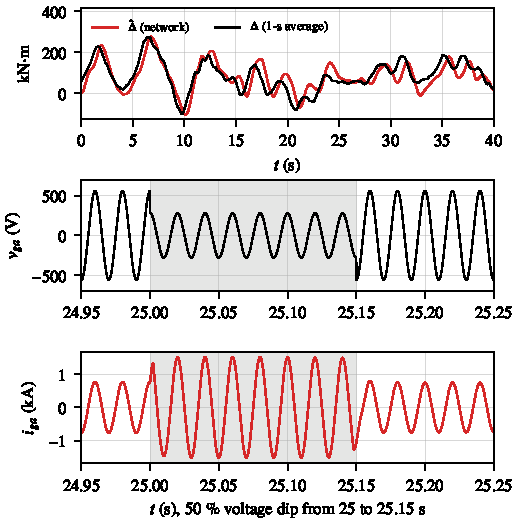
\includegraphics[width=\columnwidth]{grid.pdf}
\caption{Robustness case: network output $\hat\Delta$ and actual uncertainty $\Delta$ (1-s average), and
grid voltage and current of phase $a$ during the 50\,\% voltage dip.}
\label{fig:grid}
\end{figure}

These results are obtained with the average converter model and an ideal PLL; the switching ripple and
the PLL dynamics are not represented.

\section{Conclusion}
A 2~MW direct-drive PMSG wind energy conversion system was modeled from the wind to the grid in the
receptor convention, with an exact power balance that verifies the signs of the model. Its control
combines flatness for the speed and DC-link energy loops, passivity-based control for the currents of
both converters, and an RBF network adapted by a Lyapunov law that compensates the aerodynamic-torque and
parameter uncertainty. In simulation, all the controlled variables track their references, the DC-link
voltage remains within 1.7~V of 1200~V outside the grid dip, and the network reduces the speed tracking
error by 27 to 49\,\% at the price of a slightly more active torque, with the same captured energy.

\section*{Conflict of Interest}
The authors declare there are no conflicts of interest.

\begin{thebibliography}{99}
\bibitem{iea2024} International Energy Agency (IEA), \emph{World Energy Outlook 2024}, Paris, France, 2024.
\bibitem{gwec2024} Global Wind Energy Council (GWEC), \emph{Global Wind Report 2024}, Brussels, Belgium, 2024.
\bibitem{polinder2013} H. Polinder, J. A. Ferreira, B. B. Jensen, A. B. Abrahamsen, K. Atallah, and
R. A. McMahon, ``Trends in wind turbine generator systems,'' \emph{IEEE J. Emerg. Sel. Topics Power
Electron.}, vol.~1, no.~3, pp.~174--185, Sep. 2013.
\bibitem{wu2011} B. Wu, Y. Lang, N. Zargari, and S. Kouro, \emph{Power Conversion and Control of Wind
Energy Systems}. Hoboken, NJ, USA: Wiley-IEEE Press, 2011.
\bibitem{chinchilla2006} M. Chinchilla, S. Arnaltes, and J. C. Burgos, ``Control of permanent-magnet
generators applied to variable-speed wind-energy systems connected to the grid,'' \emph{IEEE Trans.
Energy Convers.}, vol.~21, no.~1, pp.~130--135, Mar. 2006.
\bibitem{yazdani2010} A. Yazdani and R. Iravani, \emph{Voltage-Sourced Converters in Power Systems:
Modeling, Control, and Applications}. Hoboken, NJ, USA: Wiley-IEEE Press, 2010.
\bibitem{fliess1995} M. Fliess, J. L\'evine, P. Martin, and P. Rouchon, ``Flatness and defect of
non-linear systems: Introductory theory and examples,'' \emph{Int. J. Control}, vol.~61, no.~6,
pp.~1327--1361, 1995.
\bibitem{aimene2022} M. Aimene, A. Payman, and B. Dakyo, ``Comparative study between flatness-based and
field-oriented control methods of a grid-connected wind energy conversion system,'' \emph{Processes},
vol.~10, no.~2, Art.~no.~378, 2022, doi: 10.3390/pr10020378.
\bibitem{thounthong2010} P. Thounthong, S. Pierfederici, and B. Davat, ``Analysis of differential
flatness-based control for a fuel cell hybrid power source,'' \emph{IEEE Trans. Energy Convers.},
vol.~25, no.~3, pp.~909--920, Sep. 2010.
\bibitem{ortega1998} R. Ortega, A. Lor\'ia, P. J. Nicklasson, and H. Sira-Ram\'irez,
\emph{Passivity-Based Control of Euler-Lagrange Systems}. London, UK: Springer, 1998.
\bibitem{lewis1999} F. L. Lewis, S. Jagannathan, and A. Ye\c{s}ildirek, \emph{Neural Network Control of
Robot Manipulators and Nonlinear Systems}. London, UK: Taylor \& Francis, 1999.
\bibitem{heier2014} S. Heier, \emph{Grid Integration of Wind Energy: Onshore and Offshore Conversion
Systems}, 3rd ed. Chichester, UK: Wiley, 2014.
\bibitem{hasan2021} S. M. M. Hasan and A. H. M. Shatil, ``Design and comparison of grid connected
permanent magnet synchronous generator non-salient pole and salient pole rotor wind turbine,''
\emph{AIUB J. Sci. Eng.}, vol.~20, no.~2, pp.~40--46, 2021.
\bibitem{rolan2009} A. Rolan, A. Luna, G. Vazquez, D. Aguilar, and G. Azevedo, ``Modeling of a variable
speed wind turbine with a permanent magnet synchronous generator,'' in \emph{Proc. IEEE Int. Symp. Ind.
Electron. (ISIE)}, Seoul, Korea, 2009, pp.~734--739, doi: 10.1109/ISIE.2009.5218120.
\bibitem{regani2026} S. Regani, M. Messadi, and K. Kemih, ``A novel chaos control approach with
adaptive ANN compensation for a DFIG-based wind turbine,'' \emph{Mathematics}, under review, 2026.
\bibitem{khalil2002} H. K. Khalil, \emph{Nonlinear Systems}, 3rd ed. Upper Saddle River, NJ, USA:
Prentice Hall, 2002.
\end{thebibliography}

\end{document}
